
%----------------------------------------------------------------------------------------
%	PACKAGES AND THEMES
%----------------------------------------------------------------------------------------

\documentclass{beamer}
\mode<presentation> {
\usetheme{Berlin}
}
\AtBeginSection[]{
  \begin{frame}
  \vfill
  \centering
  \begin{beamercolorbox}[sep=8pt,center,shadow=true,rounded=true]{title}
    \usebeamerfont{title}\insertsectionhead\par%
  \end{beamercolorbox}
  \vfill
  \end{frame}
}
\usepackage{graphicx} % Allows including images
\usepackage{booktabs} % Allows the use of \toprule, \midrule and \bottomrule in tables

%----------------------------------------------------------------------------------------
%	TITLE PAGE
%----------------------------------------------------------------------------------------
\titlegraphic{
\includegraphics[width=3.5cm]{photo/logo}}

\title{IT-Projekt \\ Autonomously driving Remote Control Car} % The short title appears at the bottom of every slide, the full title is only on the title page
\author{Bohnstedt Timo ,
      L\"ohr Tim and Palpanes Ionannis\\%
      } 
\institute[Computer Science| Prof. Dr. Florian Gallwitz] % Your institution as it will appear on the bottom of every slide, may be shorthand to save space
{
Georg Simon Ohm University of Applied Science\\ % Your institution for the title page
\medskip
\textit{IT Project Presentation} 
}
\date{\today} % Date, can be changed to a custom date
%----------------------------------------------------------------------------------------
\begin{document}

\begin{frame}
\titlepage % Print the title page as the first slide
\end{frame}
%----------------------------------------------------------------------------------------
\begin{frame}
\frametitle{Overview} % Table of contents slide, comment this block out to remove it
\tableofcontents % Throughout your presentation, if you choose to use \section{} and \subsection{} commands, these will automatically be printed on this slide as an overview of your presentation
\end{frame}
%
%----------------------------------------------------------------------------------------
%	PRESENTATION SLIDES
%----------------------------------------------------------------------------------------

%------------------------------------------------
\section{Background}
%------------------------------------------------

\begin{frame}
\frametitle{Start of an equally simple business}
"Brian thought of a way to make a few bucks - turning
our place into \textit{designers bed and breakfast} - offering young
designers who come to town a place to cra during the 4 day
event, complete with wireless Internet, a small desk space,
sleeping mat, and breakfast each morning. Ha!
joe”
\begin{figure}
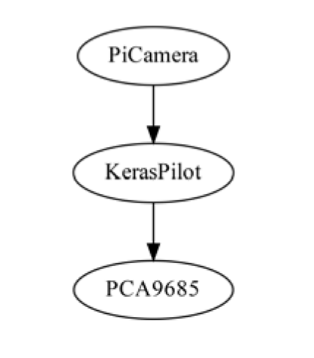
\includegraphics[width=0.4\linewidth]{photo/autonom}
\end{figure}
\end{frame}

%------------------------------------------------

\begin{frame}
\frametitle{Basics}
Airbnb is a model based on share economy. Everyone who owns an apartment can rent it out for travelers as a resting place, where it feels like home. There is a Mobile app/website: online platform to match demand and supply Listings (check in and check out: demand for short period rent apartment) .
\begin{figure}
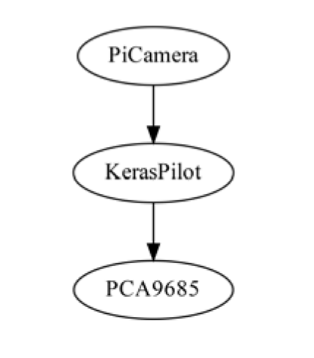
\includegraphics[width=0.4\linewidth]{photo/autonom}
\end{figure}
\end{frame}

%------------------------------------------------
\section{Literature Survey}
%---------------------------------------------
\begin{frame}
\frametitle{General Methology}
Using data analysis and show how it can be used to improve the marketing of Airbnb in Seattle according to each policy of the marketing-mix.
\end{frame}
%
%------------------------------------------------
%
\begin{frame}
\frametitle{Marketing}
\begin{columns}[c] % The "c" option specifies centered vertical alignment while the "t" option is used for top vertical alignment

\column{.45\textwidth} % Left column and width
\textbf{The 4 P's of the Marketing-Mix}
\begin{enumerate}
\item Product
\item Price
\item Promotion
\item Place
\end{enumerate}

\column{.5\textwidth} % Right column and width

\begin{block}{Definition Marketing}
Marketing is about the firm’s effort to address customer needs and expectations, which influences the demands made by the customers on the product and need to be fulfilled by the product.
\end{block}
\end{columns}
\end{frame}

%------------------------------------------------

\begin{frame}
\frametitle{How to use Data Analysis to improve the Airbnb Marketing?}
\begin{itemize}
\item \textbf{Descriptive analysis:} Reviews, locations, review and price correlation, details of listings and price correlation
\item \textbf{Descriptive analysis:} Predict the number of customer
\item \textbf{Optimization:} Optimize the booking of listings 
\item \textbf{Adaptive learning:} Learn from the results generated and combine results to give out suggestion in marketing campaigns may hold by Airbnb
\end{itemize}
\end{frame}

%------------------------------------------------
\section{Hardware}
%--------------------------------------------

\begin{frame}
\frametitle{Remote Control Car}
\begin{itemize}
\item Model car with a servomotor and electronic speed control (ESC)
\item Weights only 1,88kg
\item Easy to attach Raspberry Pi 3B+ and SunFounder Servodriver onto it
\end{itemize}
\begin{figure}
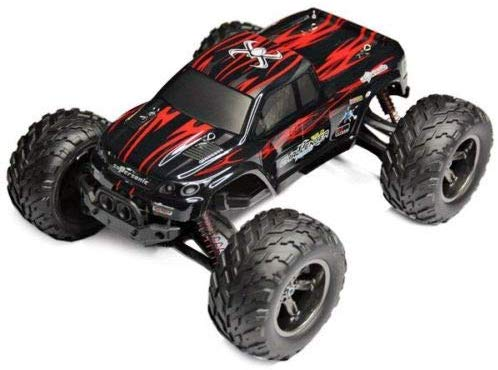
\includegraphics[width=0.4\linewidth]{photo/car.jpg}
\end{figure}
\end{frame}
%------------------------------------------------
\begin{frame}
\frametitle{Raspberry Pi 3B+ - Part l}
\begin{itemize}
\item Chosen over NVIDIA's Drive PX for this project, because the weight and power are suiting  better
\item 1.4GHz CPU to apply the Deep Learning to the captured images
\item 16GB SanDisk SD-Card storage with Raspian Stretch Lite
\item Powered through a Powerbank attached onto the RC-Car
\begin{figure}
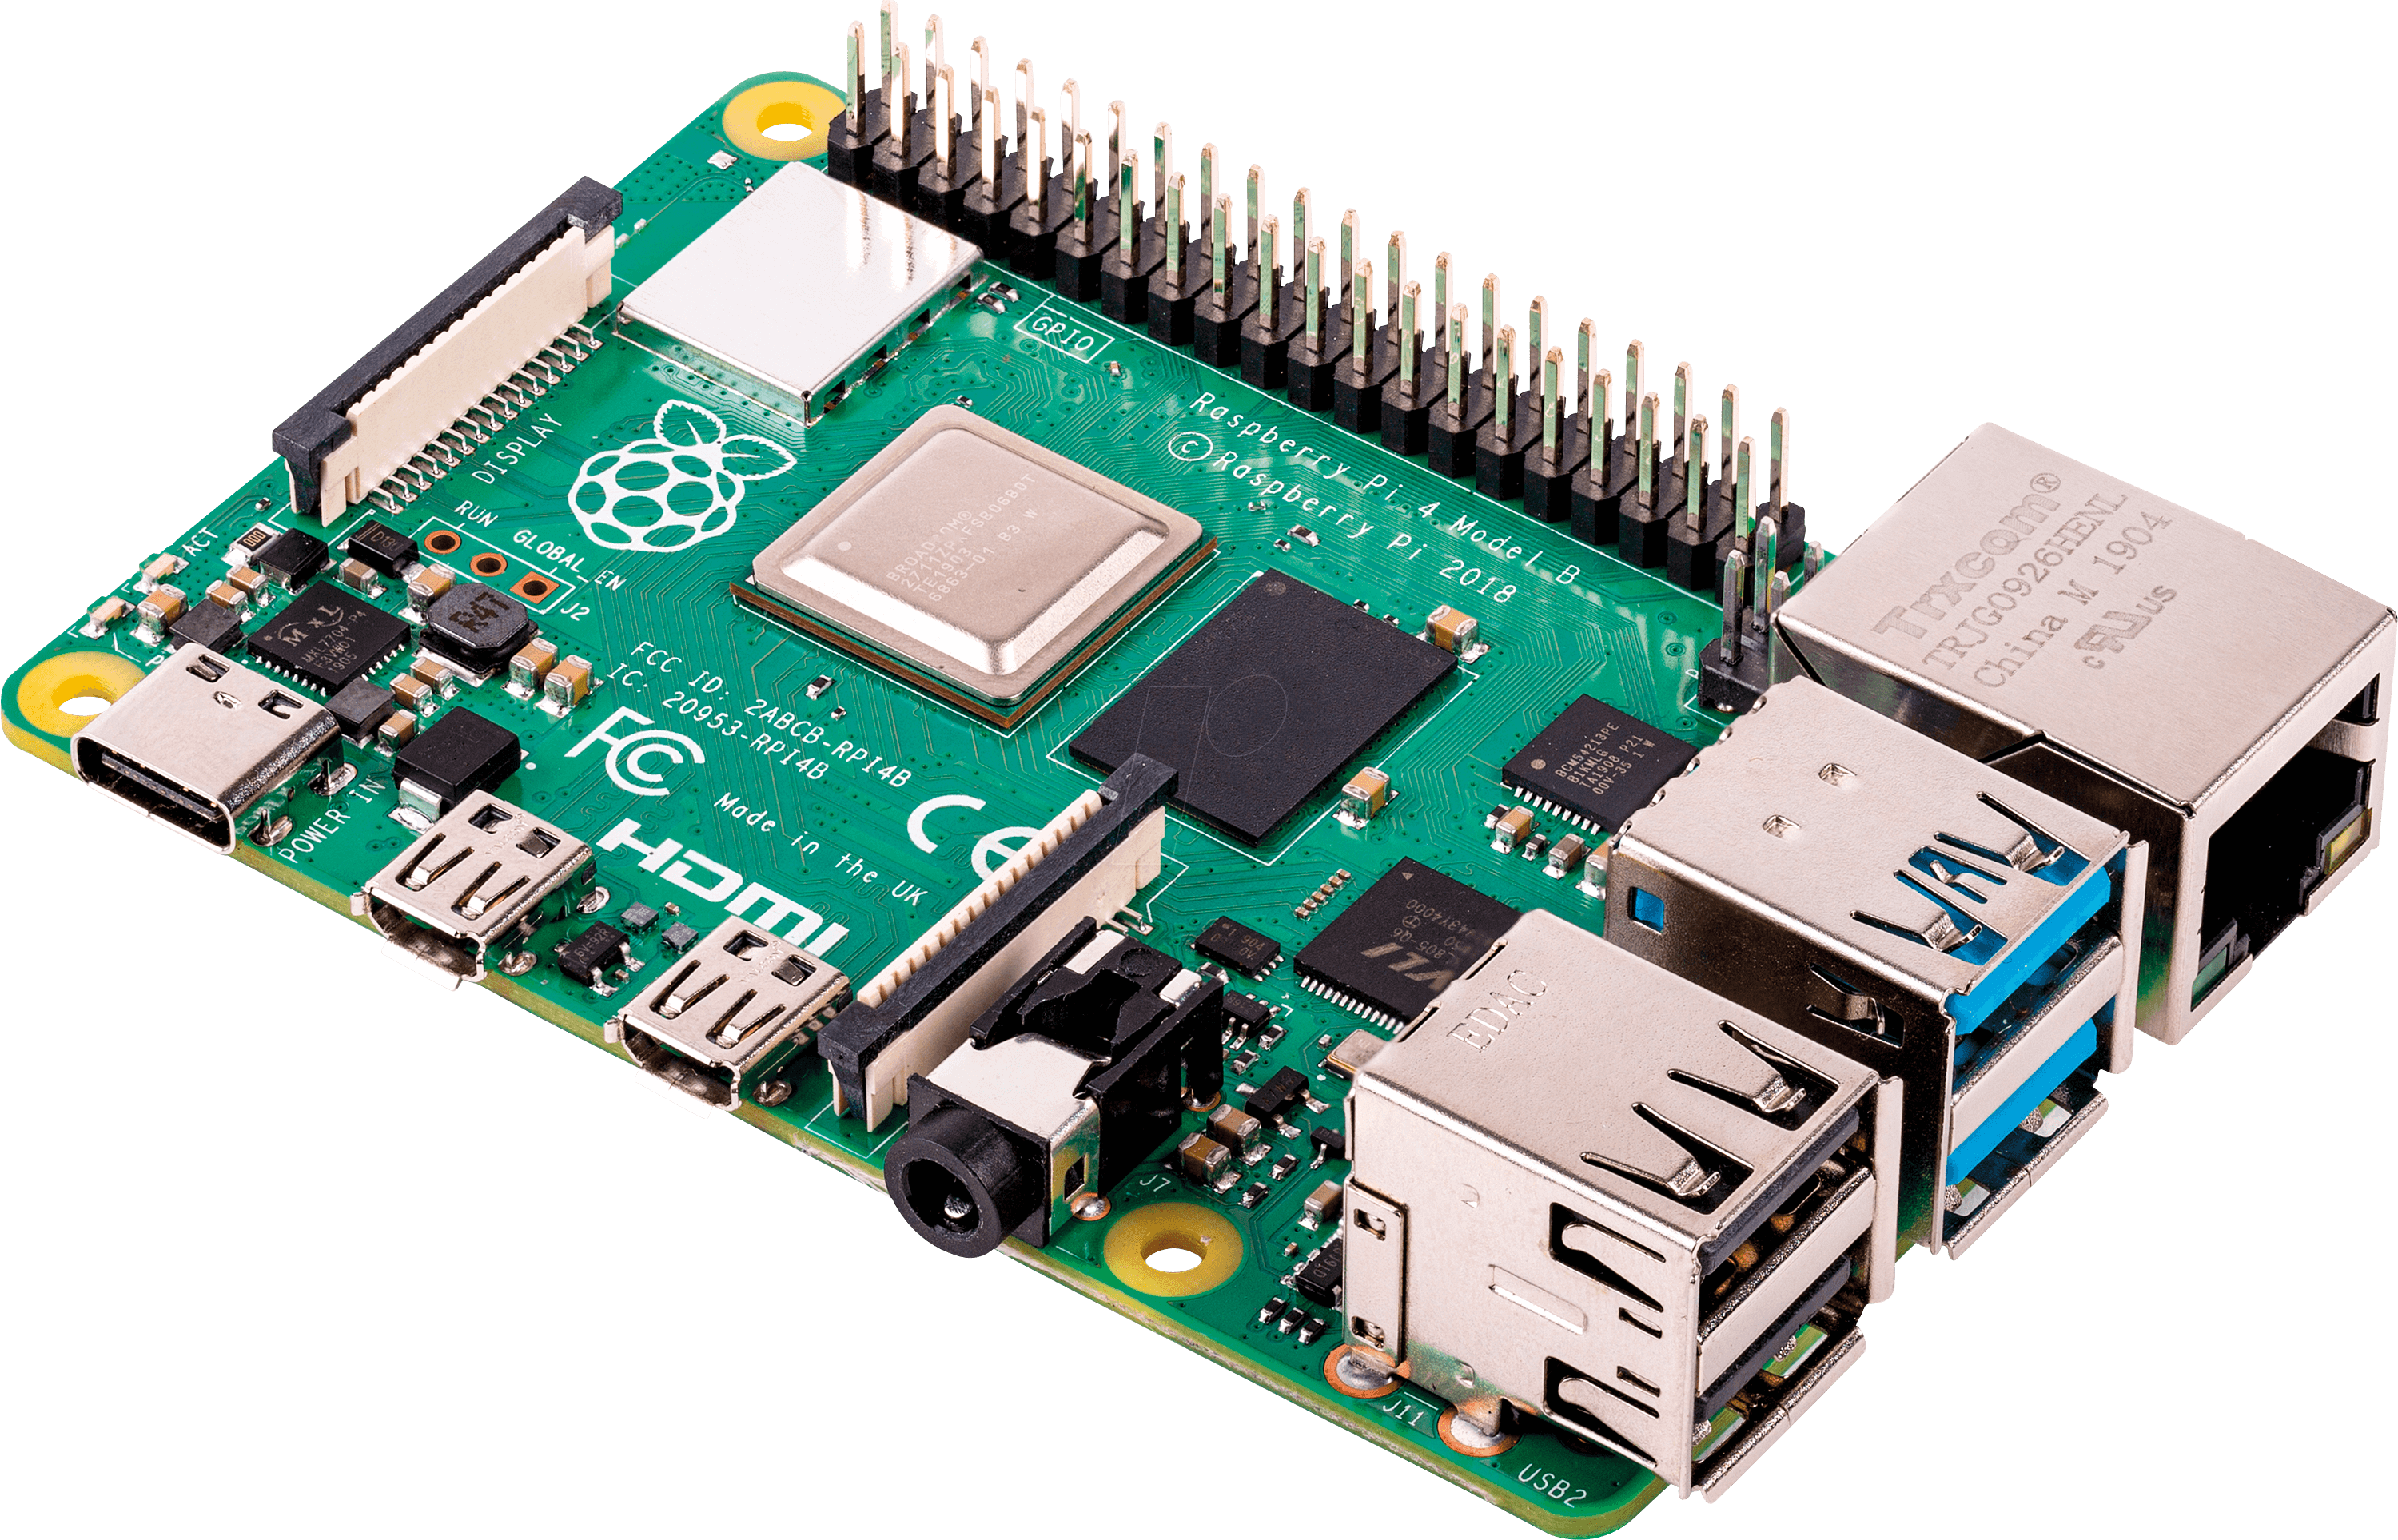
\includegraphics[width=0.4\linewidth]{photo/raspi}
\end{figure}
\end{itemize}
\end{frame}

%------------------------------------------------

\begin{frame}
\frametitle{Raspberry Pi 3B+ - Part ll}
\begin{columns}[c] % The "c" option specifies centered vertical alignment while the "t" option is used for top vertical alignment
\column{.45\textwidth} % Left column and width
\begin{itemize}
\item For our purpose, we use the Rasp- berry Pi Camera Module 8MP v2.1. It can capture pictures with 1080p and 8-megapixel focus \\
\item Connector on the Raspberry Pi 3B+ with a 15 Pin Ribbon Cable
\end{itemize}

\column{.45\textwidth} % Right column and width
PiCamera Module
\begin{figure}
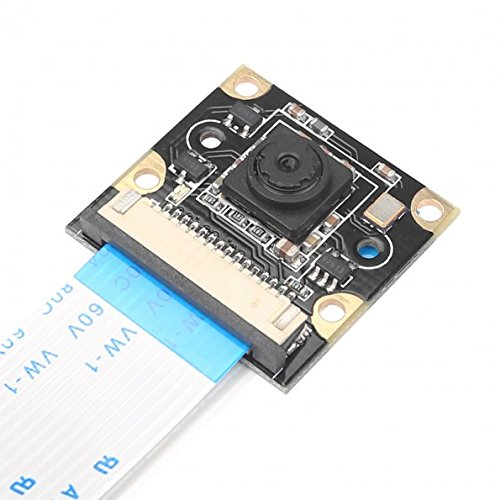
\includegraphics[width=0.7\linewidth]{photo/camera.jpg}
\end{figure}
\end{columns}

\end{frame}

%------------------------------------------------

\begin{frame}
\frametitle{Servodriver}
From SunFounder, model \textit{PCA9685}
\begin{itemize}
\item Cheap price: approximately ~13
\item Provides Pulse width modulation (PWM) to apply remote steering through the Raspberry Pi 3B+
\item Powered with 3-5V from the Raspberry Pi 3B+
\end{itemize}
\begin{figure}
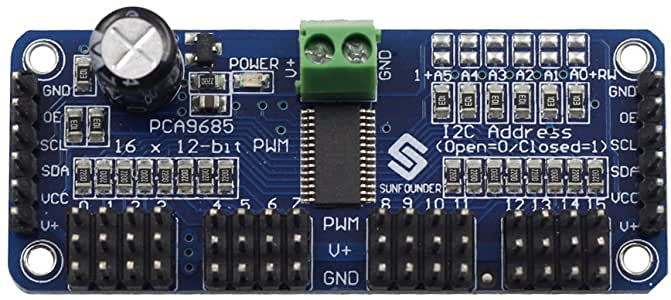
\includegraphics[width=0.4\linewidth]{photo/sunfounder.jpeg}
\end{figure}
\end{frame}

%------------------------------------------------

\begin{frame}
\frametitle{Cable Management - Part I}
\begin{block}{Raspberry Pi 3B+ to Servodriver}
8 Pin's need to be connected. 
\begin{itemize}
\item Ground GND
\item Power VCC 5 Volt
\item 2x3 Pin's for the steering and throtteling
\end{itemize}
\end{block}

\begin{block}{Servodriver to Servomotor}
Four Pin's need to be connected. 
\begin{itemize}
\item Ground GND
\item Power VCC 5 Volt
\item 2 Pin's for the steering and throtteling
\end{itemize}
\end{block}
%
\end{frame}

%------------------------------------------------

\begin{frame}
\frametitle{Cable Management - Part ll}
\begin{figure}
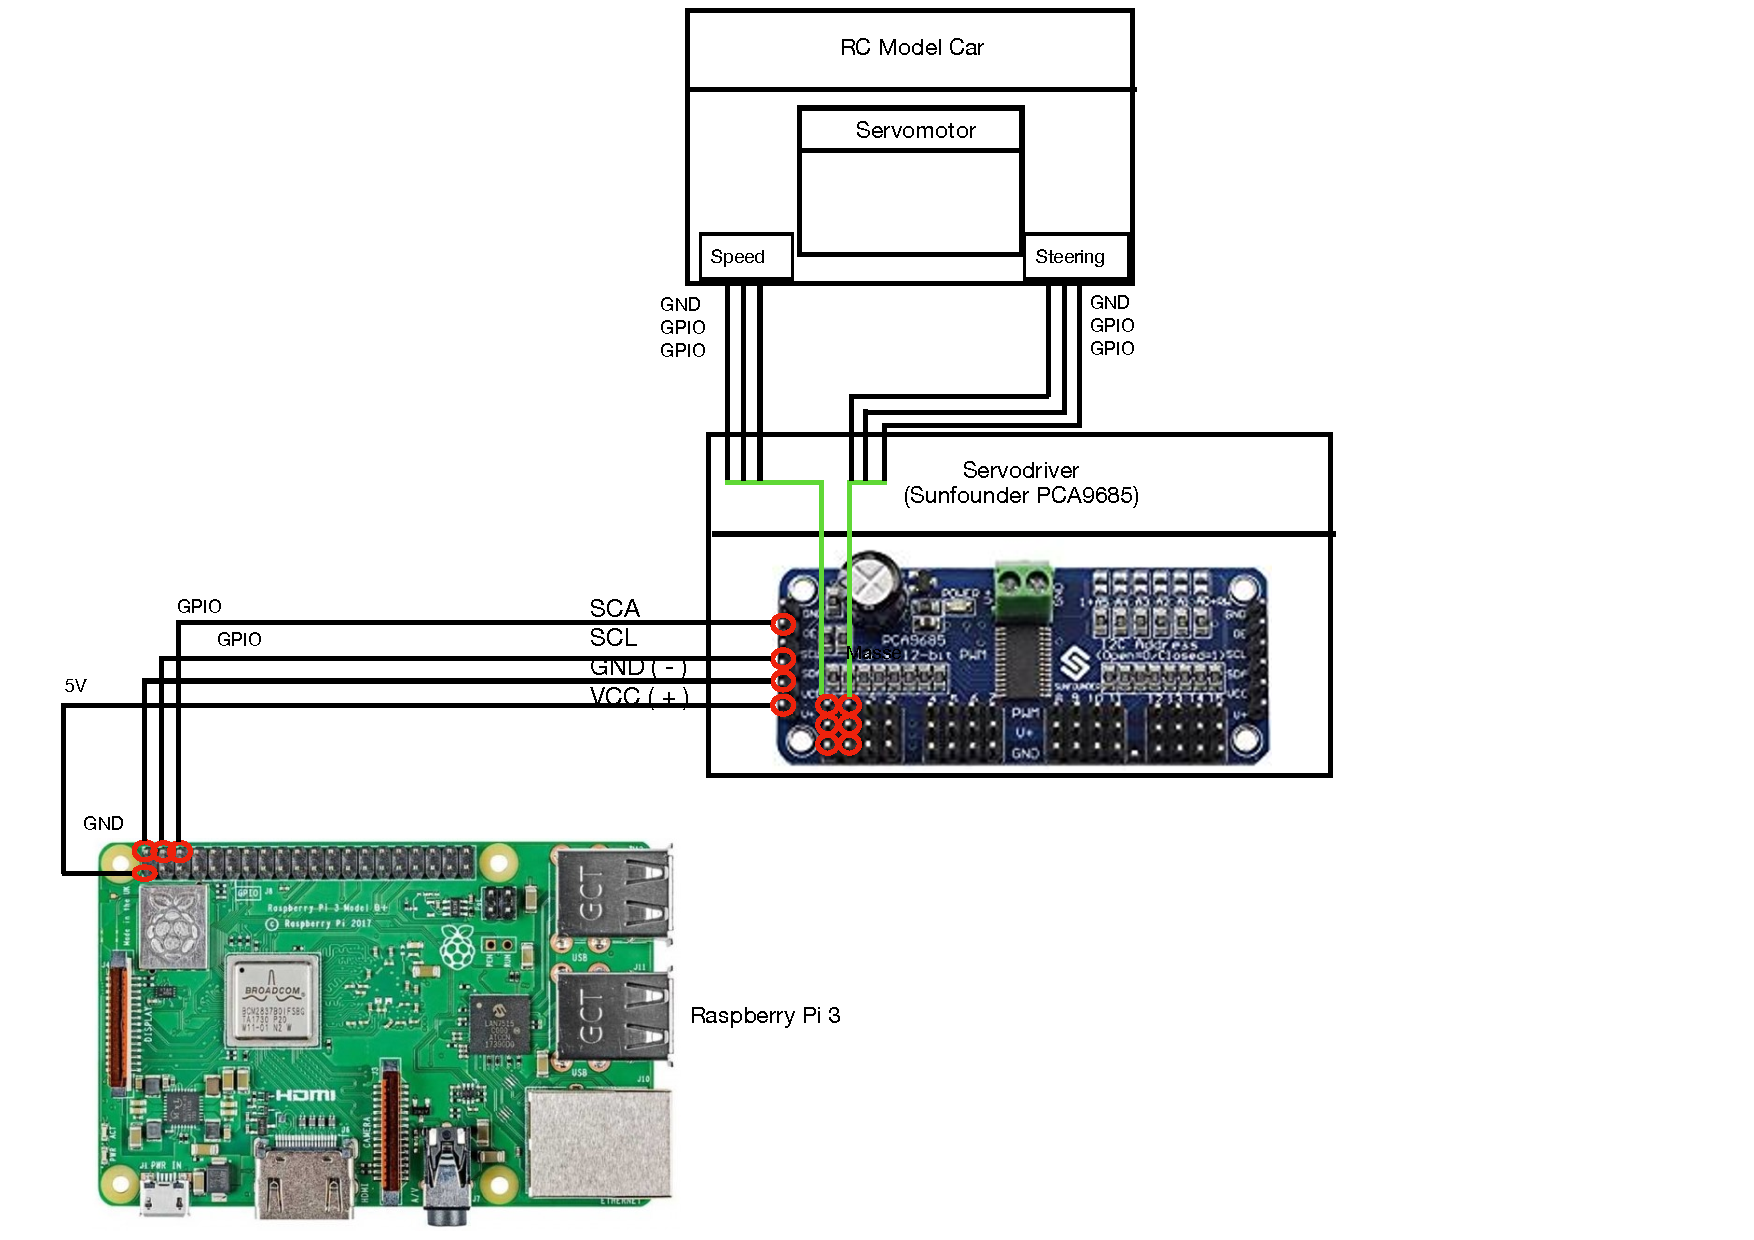
\includegraphics[width=0.7\linewidth]{photo/ebene2.pdf}
\end{figure}
\end{frame}

%------------------------------------------------
\section{Software}
%------------------------------------------------

%------------------------------------------------

\begin{frame}
\frametitle{Software Architecture - Python Files}
The Donkey Self-Driving Car Project is the basis for our group Project. The Filesystem is: \\
\begin{itemize}
\item Management: Start the Webserver
\item Parts: Controls the single parts, e.g. Camera, Steering, Throttle, ..
\item Templates: Web Templates for the Webserver
\item Test: Start the environment without error's
\end{itemize}
\end{frame}

%------------------------------------------------

%------------------------------------------------

\begin{frame}
\frametitle{Python Tornado Webserver}
\begin{figure}
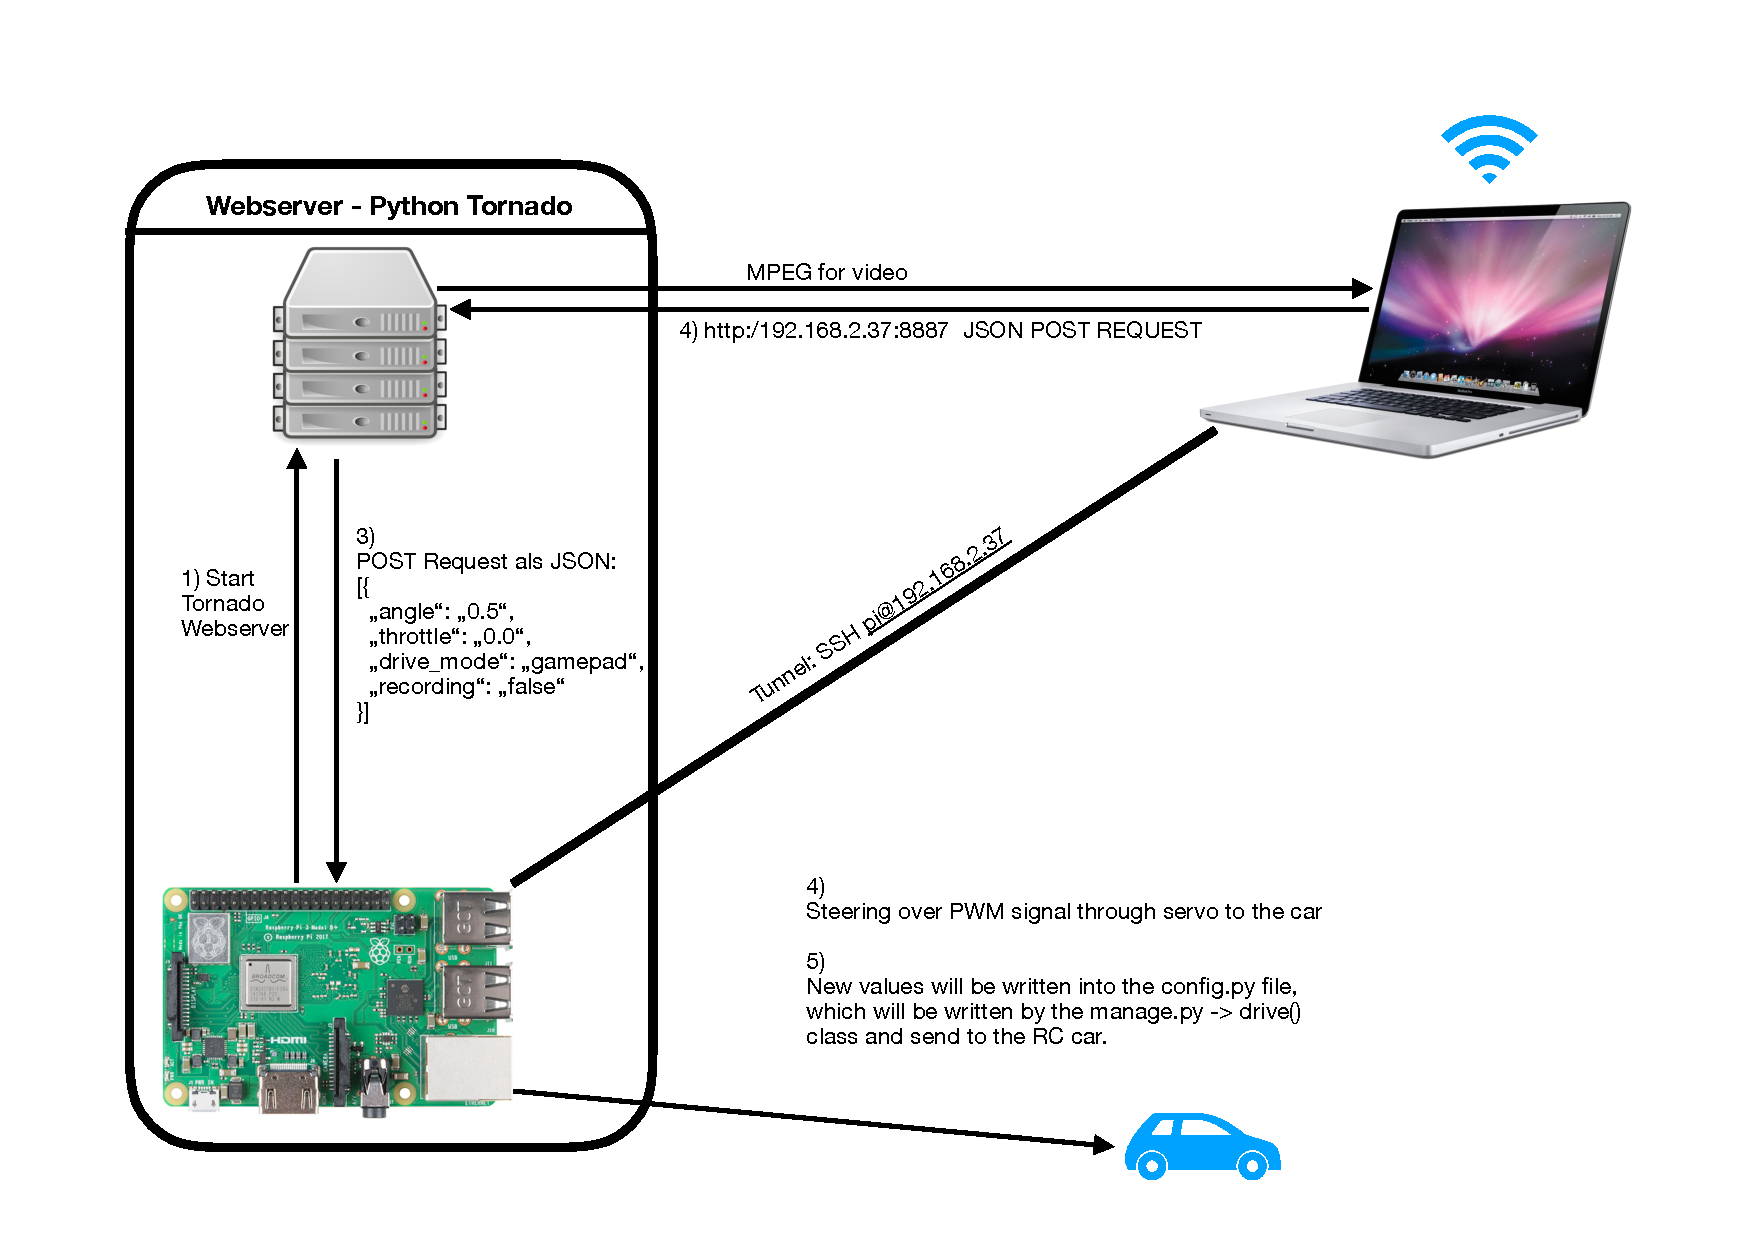
\includegraphics[width=0.9\linewidth]{photo/webserver.pdf}
\end{figure}
\end{frame}

%------------------------------------------------

\begin{frame}
\frametitle{Training the model with Unity}
\begin{columns}[c] % The "c" option specifies centered vertical alignment while the "t" option is used for top vertical alignment

\column{.45\textwidth} % Left column and width
\begin{itemize}
\item For capturing enough images, someone from the DonkeyCar community programmed a Unity Game.
\item Simulator of the real word with lines on the border of the track for the image recognition task
\end{itemize}

\column{.45\textwidth} % Right column and width
Snapshot from the Simulation
\begin{figure}
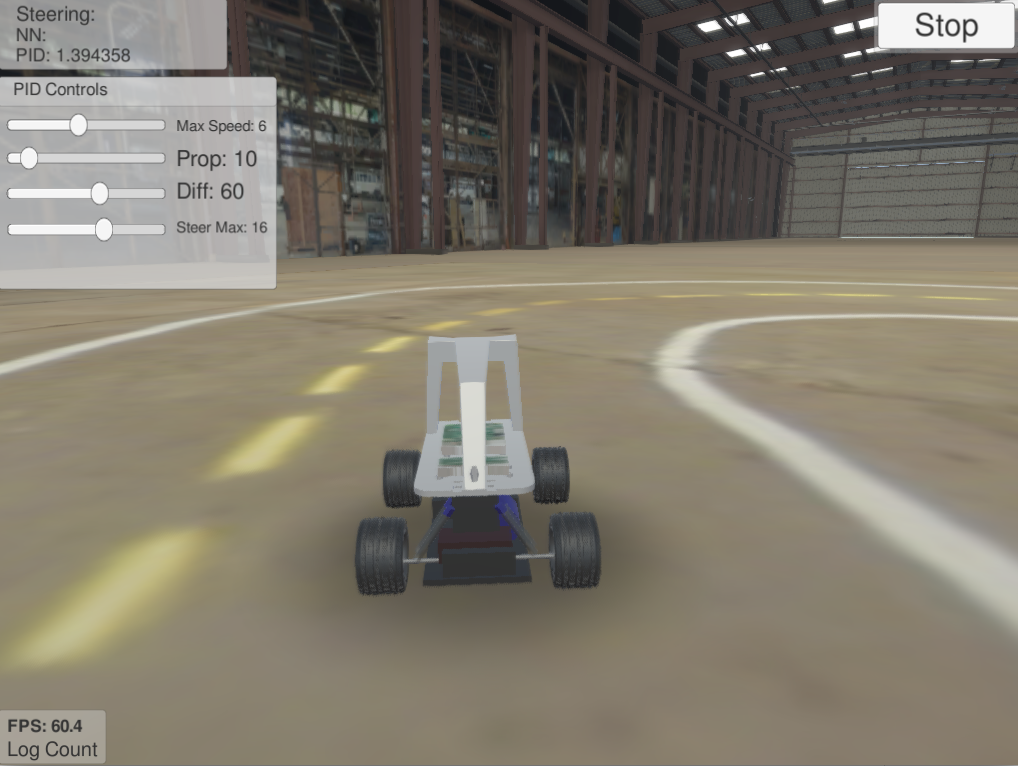
\includegraphics[width=0.9\linewidth]{photo/unity}
\end{figure}
\end{columns}
\end{frame}
%------------------------------------------------

\section{Machine Learning}
%--------------------------------------------
\begin{frame}
The team around Josh Keating reached a mean absolute error between 32\$ to 35\$
\begin{itemize}
\item Our network design was way to simple
\item We didn't include the important neighbourhood feature
\item Our result with our LSTM neural network was 64.04\$ (MSA)
\item Nevertheless, our best model was the linear regression with a MAE of 43.89\$
\end{itemize}
\end{frame}

%------------------------------------------------

\begin{frame}
\frametitle{Which facts lessors need to address in their description to raise the interest of potential customer, who ‘fit’ the vibe of the neighborhood and set their focus on the same aspects as former customers of these apartments?}
As shown in the word cloud:
\begin{itemize}
\item The six most reviewed cities are Capitol Hill, Ballard, Queen Anne, Belltown, Minor, Wallingford 
\item All cities have the words walk, park and restaurant written in big
\item The word “downtown” is also used often
\item For Minor, the word “lake” is very important
\item Interestingly, the word “Washington” is important for the cities Minor and Capitol Hill
\end{itemize}
\end{frame}

%------------------------------------------------

\begin{frame}
\frametitle{Which price can be charged for an apartment with certain characteristics?}
Heatmap: Correlation between features and price
\begin{figure}
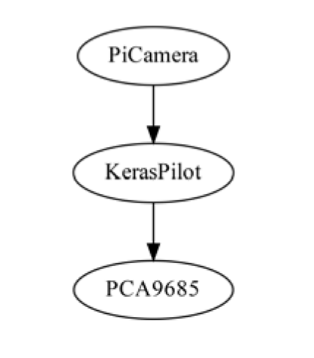
\includegraphics[width=0.8\linewidth]{photo/autonom}
\end{figure}
\end{frame}
%------------------------------------------------
\begin{frame}
\frametitle{Which price can be charged for an apartment with certain characteristics?}
As shown in the heatmap from the previous slide, there is a clear correlation between number of bedrooms and price.\\More features with correlate with the price are the beds, bathrooms, room type and guests included.
\begin{figure}
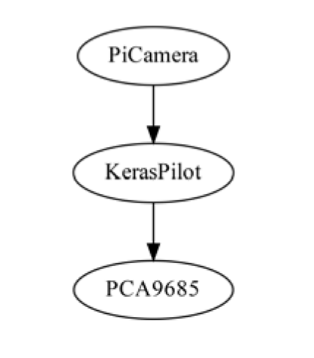
\includegraphics[width=0.8\linewidth]{photo/autonom}
\end{figure}
\end{frame}
%------------------------------------------------
\begin{frame}
\frametitle{Which price can be charged for an apartment with certain characteristics?}
Another big indicatior is the \textbf{season}. As shown in the figure below there is a strong fluctuation between the prices and the seasons.\\ So, we need to adapt our price on the current month.
\begin{figure}
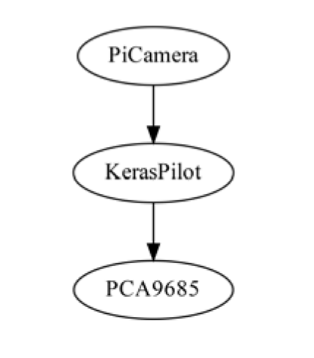
\includegraphics[width=0.8\linewidth]{photo/autonom}
\end{figure}
\end{frame}
%------------------------------------------------
\begin{frame}
\frametitle{When can lessors increase the price per night for their apartment and when should they lower it?}
\begin{itemize}
\item Price increase from January and July from 120\$ to 150\$
\item Price decrease until November to 135\$
\item We can detect an increasing demand for flats in summer time and Christmas with a correlation of an increasing price
\end{itemize}
\begin{figure}
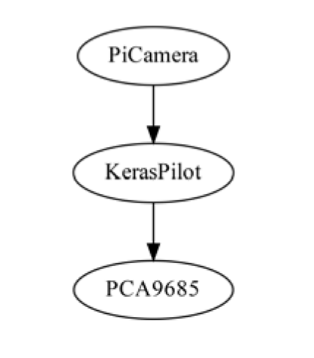
\includegraphics[width=0.8\linewidth]{photo/autonom}
\end{figure}
\end{frame}
%------------------------------------------------
\begin{frame}
\frametitle{What is a good point in time to start a marketing campaign?}
We can see clearly the high fluctuation of visitors on a weekly basis, but it is also obvious that it correlates with the picture before.\\It could be explained by people are more likely to travel on weekends than on weekdays
\begin{figure}
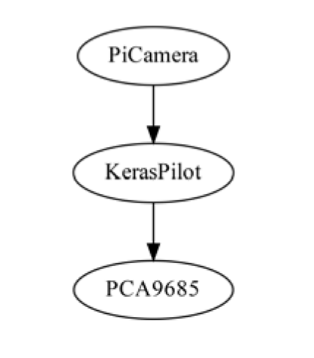
\includegraphics[width=0.8\linewidth]{photo/autonom}
\end{figure}
\end{frame}
%------------------------------------------------
\section{Deep Learning}
%------------------------------------------------
\begin{frame}
\frametitle{Our Findings and Impacts}
\begin{itemize}
\item The reviews are the most important factor of the costumers decision
\item Lessors should ask their guests to leave a review after staying at the 
\item Lessors should consider to update their description with attractive places nearby. For example a lake, park or restaurants.
\end{itemize}
\end{frame}
%------------------------------------------------
\begin{frame}
\frametitle{Our Findings and Impacts}
\begin{itemize}
\item Another big factor is how long the host has been acted and how many listings the host has
\item Hosts should try to increase their response time
\item Obviously providing more bathrooms or bedrooms leads to rent the flat for a higher price
\end{itemize}
\end{frame}
%------------------------------------------------
\section{Autonomously Driving}
%------------------------------------------------
\begin{frame}
\frametitle{Keras Pilot - Part I}
The Keras Pilot (\textit{.h5} Format) is stored on the Raspberry Pi. 

\begin{itemize}
\item The image captured with the PiCamera are 160x120x3 Pixels
\item They pass through the follwing Neural Network
\item The Output in the last fully connected Layer is \\ (\textit{angle\_out} and \textit{throttle\_out})
\end{itemize}

\begin{figure}
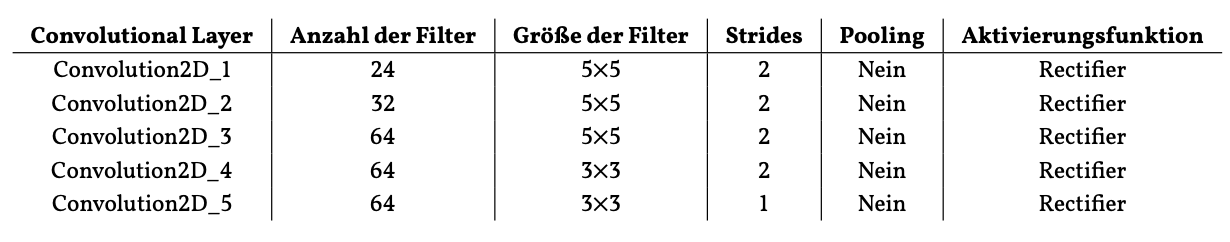
\includegraphics[width=1\linewidth]{photo/cnn_table}
\end{figure}

\end{frame}
%---------------------------------------------

\begin{frame}
\frametitle{Keras Pilot - Part ll}
Connection with the PiCamera Module:
\begin{columns}[c] % The "c" option specifies centered vertical alignment while the "t" option is used for top vertical alignment
\column{.45\textwidth} % Left column and width
\begin{itemize}
\item We use 20 frames per second (FPS)
\item We use Tensorflow 1.1.17 for version compatibility
\item According to that, the car changes 20 times per second the angle
\item The throttle is fix, because of the space limitation
\end{itemize}

\column{.45\textwidth} % Right column and width

\begin{center}
	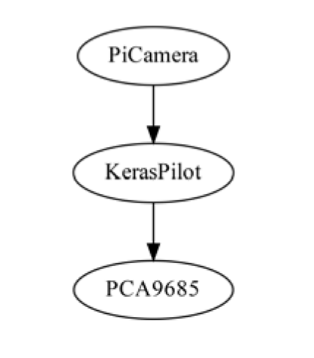
\includegraphics[width=4cm]{photo/autonom}
\end{center}

\end{columns}
\end{frame}
%----------------------------------------------------------------------------------------

\section{Evaluation}
%------------------------------------------------
\begin{frame}
\frametitle{Evaluation - Part l}
\begin{columns}[c] % The "c" option specifies centered vertical alignment while the "t" option is used for top vertical alignment
\column{.45\textwidth} % Left column and width
\begin{block}{Evaluation}
Even though CNN perform a really good result in the computer vision field, it is still quite hard to decompse the decisions and the filters to understand the blackbox behind. For this reason visualized one decision by plotting the occlusion maps (next page) based on this criterion function
\end{block}

\column{.45\textwidth} % Right column and width
The criterion function:
\begin{equation}
O_{i,j}= \begin{cases}
    0,& \text{if } abs(\hat{y}_{i,j} - y) > \epsilon\\
    1              & \text{otherwise} \end{cases}
\end{equation}
\end{columns}

\end{frame}
%---------------------------------------------

\begin{frame}
\begin{block}{Evaluation - Part ll: Occlusion maps generated out of the CNN layers from section \textit{Autonomously Driving - Keras Pilot (Part l)}}

\begin{center}
	
\includegraphics[width=5cm]{photo/filter}
\end{center}
\begin{center}
Not interpolated filter and gray with bilinear interpolation
\end{center}

\begin{center}
	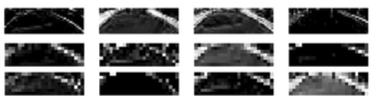
\includegraphics[width=6cm]{photo/activations}
\end{center}
\begin{center}
Activation features after each Layer of the NN respectively
\end{center}
\end{block}


\end{frame}

%------------------------------------------------

\begin{frame}
\frametitle{Conclusion}

\begin{block}{Final Thoughts}
The project was challenging, but all of us learned a lot during this 2 semester long process of building up this project. While doing this project, Tensorflow 2.0 was released and this changed a lot. We needed to adjust constantly, because the Tech-research is so fast.
In conclusion, we had a great time and are eager to dive deeper into Deep Learning!
\end{block}

\begin{block}{Acknowledgement}
The authors would like to thank Prof Dr. Florian Gallwitz from the University of Applied Science - Georg Simon OHM in Nuremberg.
\end{block}

\end{frame}

%------------------------------------------------

\begin{frame}
\frametitle{References}
\begin{itemize}
\item Github: https://github.com/bohniti/it-projekt
\item Website: https://bohniti.github.io/it-projekt/project/
\end{itemize}

\begin{block}{Sources}
All of our sources are listed in the project paper on Github.
\end{block}
\begin{center}
Thanks for listening!
\end{center}
\end{frame}

%------------------------------------------------

\begin{frame}
\Huge{\centerline{The End}} 
\vspace{5mm}
\begin{center}
	
\includegraphics[width=10cm]{photo/logo}
\end{center}
\end{frame}
%----------------------------------------------------------------------------------------

\end{document} 